
Rossby-Wellen, auch planetare Wellen genannt, sind grossräumige
Wellenerscheinungen, die in erster Linie durch die Breitenabhängigkeit des
Coriolis-Parameters verursacht werden. Diese Breitenabhängigkeit wird durch den \emph{Beta-Term}
\begin{equation}
	\beta = \frac{\partial f}{\partial y}
	\label{rossby:eq:beta_term}
\end{equation}
beschrieben. Bewegt sich ein Luftpaket meridional, erfährt es eine Änderung seiner planetaren Vorticity \(f\). Unter der Erhaltung der potenziellen Vorticity erzwingt dies eine kompensierende Änderung der relativen Vorticity~\(\zeta\), was zu einer wellenförmigen Rückstellbewegung führt.
Diese Dynamik macht Rossby-Wellen zu einer direkten Konsequenz der Erhaltung der potenziellen Vorticity auf einer Kugel oder \(\beta\)-Ebene.

\subsubsection{Lineare Theorie barotroper Rossby-Wellen}

Dieser Abschnitt ist inspiriert von \cite{rossby:mueller2018}.

In Äquatornähe dominiert eine mittlere Ost–West-Strömung mit Geschwindigkeit
\(U\). Betrachten wir kleine Störungen \((u,v)\) dieser Strömung:
\begin{equation}
	u' = U + u, \quad v' = v, \quad \text{mit } |u|, |v| \ll U.
	\label{rossby:eq:perturbation}
\end{equation}
Für eine quellenfreie Strömung existiert eine Stromfunktion~$\psi$ (vgl.~Abschnitt~\ref{ueberschall:stroemungsgleichung}):
\begin{equation}
	u = -\frac{\partial \psi}{\partial y}, \quad v = \frac{\partial \psi}{\partial x}.
	\label{rossby:eq:stream_function}
\end{equation}
Die relative Vorticity ergibt sich zu
\begin{equation}
	\zeta = \frac{\partial v}{\partial x} - \frac{\partial u}{\partial y} = \Delta \psi,
	\label{rossby:eq:relative_vorticity}
\end{equation}
und die absolute Vorticity ist \(\zeta + f\) mit \(f = f(y)\). Unter der Annahme, dass die absolute Vorticity in der reibungsfreien Strömung erhalten bleibt,
\begin{equation}
	\frac{d}{dt} (\zeta + f) = 0,
	\label{rossby:eq:absolute_vorticity_conservation}
\end{equation}
und unter Verwendung der Näherungen
\[
	u \ll U, \quad \frac{\partial \zeta}{\partial y} \ll \frac{\partial f}{\partial y} = \beta, \quad v = \frac{\partial \psi}{\partial x},
\]
erhält man die linearisierte Vorticity-Gleichung
\begin{equation}
	\frac{\partial \zeta}{\partial t} + U \frac{\partial \zeta}{\partial x} + \beta \frac{\partial \psi}{\partial x} = 0.
	\label{rossby:eq:linear_vorticity_equation}
\end{equation}
Mit \(\zeta = \Delta \psi\) folgt
\begin{equation}
	\frac{\partial \Delta \psi}{\partial t} + U \frac{\partial \Delta \psi}{\partial x} + \beta \frac{\partial \psi}{\partial x} = 0.
	\label{rossby:eq:linear_vorticity_equation_psi}
\end{equation}

\subsection{Wellenlösungen\label{subsection:rossby:loesungen}}

Um die Eigenschaften der Rossby-Gleichung \eqref{rossby:eq:linear_vorticity_equation_psi}
zu verstehen, suchen wir Lösungen in Form kleiner Abweichungen,
die sich als Wellen ausbreiten. Ein naheliegender Ansatz ist eine
ebene Welle mit den Wellenzahlen $k$ (in $x$-Richtung) und $l$
(in $y$-Richtung) sowie der Kreisfrequenz $\omega$:
\begin{equation}
	\psi_{kl}(t,x,y) = \cos(kx + ly - \omega t).
	\label{rossby:ebenewelle}
\end{equation}
Damit wir diese Form in die Bewegungsgleichung einsetzen können,
benötigen wir ihre partiellen Ableitungen:
\begin{align*}
	\frac{\partial}{\partial t} \psi_{kl}(t,x,y)
	 & = \omega \sin(kx+ly-\omega t),
	\\[0.5em]
	\frac{\partial}{\partial x} \psi_{kl}(t,x,y)
	 & = -k \sin(kx+ly-\omega t),
	\\[0.5em]
	\Delta\psi_{kl}(t,x,y)
	 & = -\bigl(k^2+l^2\bigr)\cos(kx+ly-\omega t)
	= -\bigl(k^2+l^2\bigr)\psi_{kl}(t,x,y).
\end{align*}

Die Gleichung  \eqref{rossby:eq:linear_vorticity_equation_psi} lautet
\[
	\frac{\partial}{\partial t}\Delta \psi
	+ U \frac{\partial}{\partial x}\Delta \psi
	+ \beta \frac{\partial}{\partial x} \psi = 0.
\]
Für unseren Ansatz ergibt das:
\begin{align*}
	0
	 & = -\omega (k^2+l^2)\sin(kx+ly-\omega t)
	\\&\quad
	+ U k (k^2+l^2)\sin(kx+ly-\omega t)
	\\&\quad
	- \beta k \sin(kx+ly-\omega t)                                                      \\
	 & = \left( -\omega (k^2+l^2) + Uk (k^2+l^2) - \beta k \right) \sin(kx+ly-\omega t) \\
	 & = \left( (\omega - Uk)(k^2+l^2) + \beta k \right) \sin(kx+ly-\omega t).
\end{align*}
Die Funktion $\sin(kx+ly-\omega t)$ ist im Allgemeinen nicht null,
daher muss ihr Vorfaktor verschwinden:
\begin{equation}
	(\omega - Uk)(k^2+l^2) + \beta k = 0.
	\label{rossby:vorfaktor}
\end{equation}

\paragraph{Dispersionsrelation.}
Die Gleichung \eqref{rossby:vorfaktor} aufgelöst nach $\omega$ ergibt
\begin{align}
	\omega
	 & = Uk - \frac{\beta k}{k^2+l^2}.
	\label{rossby:dispersion}
\end{align}
Dies ist die Dispersionsrelation der Rossby-Wellen:
die Kreisfrequenz hängt sowohl von den Wellenzahlen
als auch vom Strömungsprofil ($U$) und von $\beta$ ab.

\paragraph{Phasengeschwindigkeit}
Die \emph{Phasengeschwindigkeit} bezeichnet die Geschwindigkeit, mit der ein
Punkt gleicher Phase (z.\,B.\ ein Wellenberg) entlang der Ausbreitungsrichtung
wandert. Für die $x$-Richtung ergibt sich
\begin{equation}
	c = \frac{\omega}{k} = U - \frac{\beta}{k^2+l^2}.
	\label{rossby:phasengeschwindigkeit}
\end{equation}
Der zweite Term repräsentiert den Einfluss der Variation des Coriolisparameters.
Da dieser Bruchterm stets positiv ist, gilt $c < U$.
Die Rossby-Wellen laufen also immer langsamer als die Grundströmung und
erscheinen relativ zu ihr nach Westen gerichtet.
Vertiefte Ausführungen dazu bietet Abschnitt 7.3.4 in \cite{rossby:mueller2018}.

\subsection{Rossby-Wellen und Wetterextreme}


Ein eindrucksvolles Beispiel für den Einfluss quasi-stationärer Rossby-Wellen
auf Extremwetterereignisse ist der Sommer 2010. In dieser Periode dominierten
atmosphärische Zirkulationsmuster mit einer Wellenzahl \(k \approx 6-8\), die zu
gleichzeitigen, aber geographisch weit entfernten Extremen führten, siehe auch Abbildung \ref{fig:rossby_2010}.


\begin{figure}
	\centering
	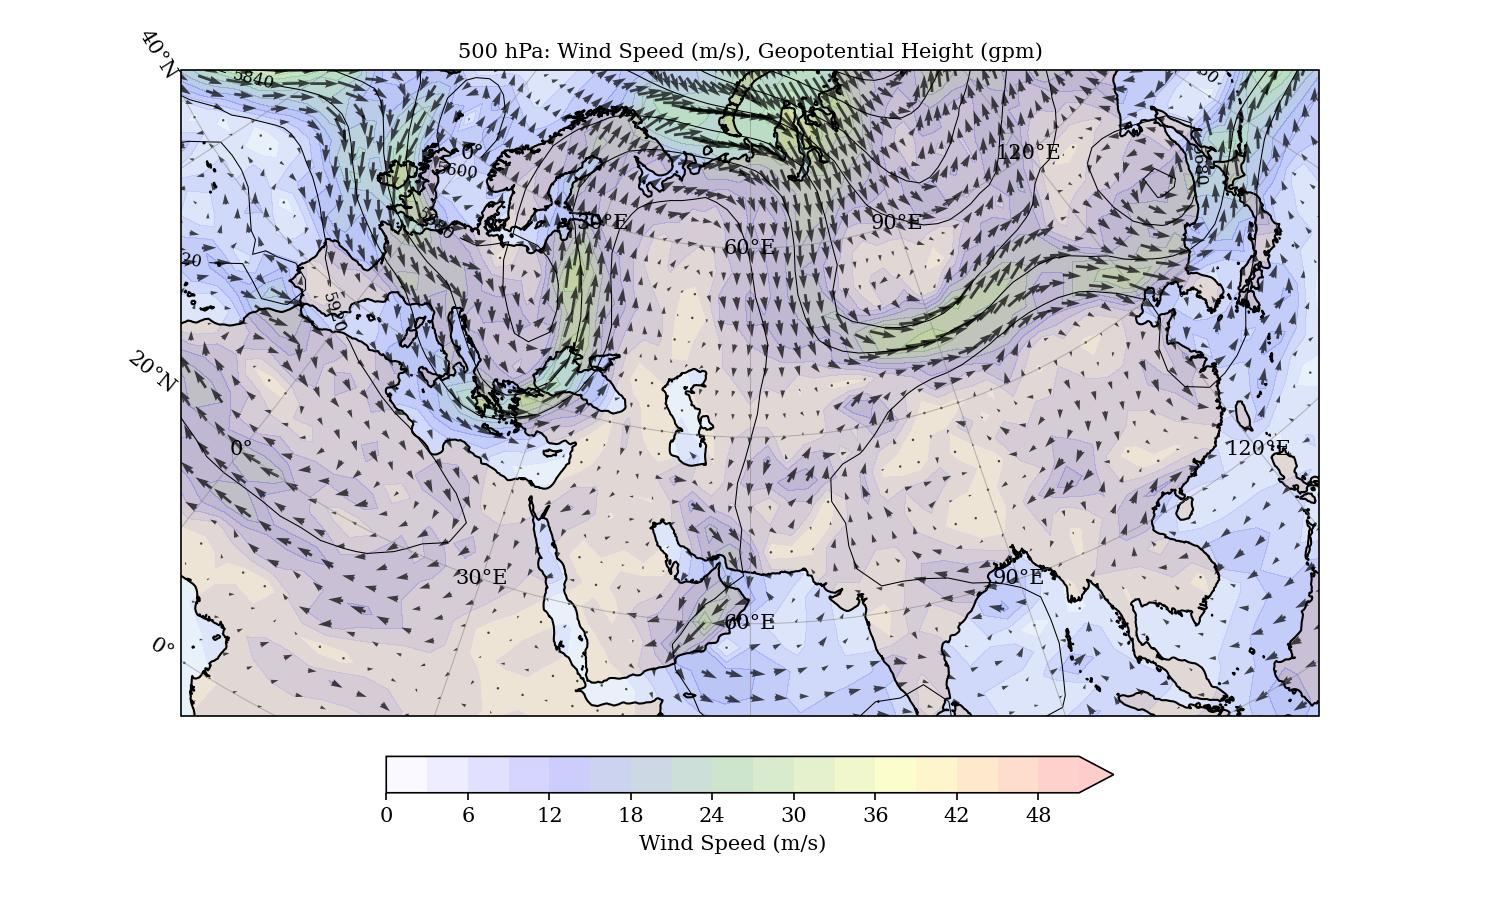
\includegraphics[width=\textwidth, trim=2cm 0cm 3cm 0cm, clip]{papers/rossby/images/data_2010_7_28_12_00_500.jpg}
	\caption{500\,hPa Windfeld am
		28.\ Juli 2010, 12:00~UTC, während der gleichzeitigen Flutereignisse in Pakistan und
		der Hitzewelle in Russland. Die Abbildung zeigt eine charakteristische Rossby-Wellenstruktur,
		die über einen längeren Zeitraum stabil blieb.}
	\label{fig:rossby_2010}
\end{figure}



\begin{figure}
	\centering
	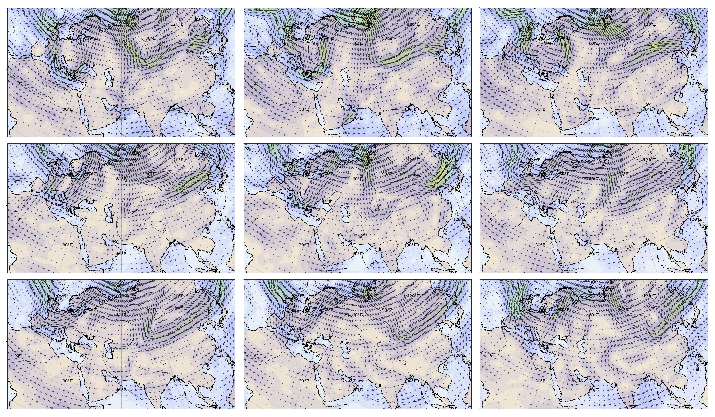
\includegraphics[width=\textwidth]{papers/rossby/images/rossby_2010.pdf}
	\caption{Abfolge der Rossby-Wellenstruktur in 500\,hPa Höhe vom 27. Juli bis 4.\ August 2010 in 24-Stunden-Schritten.
		Die Ansicht zeigt den Kontinet Aisen, die statische Wellenstruktur und die
		gleichzeitigen Extremwetterereignisse in Russland und Pakistan.
		Die Teilabbildungen sind zeilenweise von links nach rechts zu lesen, beginnend mit dem 27.\ Juli 12:00~UTC (oben links)
		bis zum 4.\ August 12:00~UTC (unten rechts).}
	\label{fig:rossby_grid_2010}
\end{figure}


Über Westrussland etablierte sich ein blockierendes Hochdruckgebiet, das über Wochen bestehen blieb und eine extreme Hitzewelle mit Temperaturen über 40\,$^\circ$C auslöste.
Die anhaltende Trockenheit begünstigte grossflächige Waldbrände und dichten Smog, besonders im Raum Moskau, mit tausenden Todesopfern.

Zur gleichen Zeit erlebte Pakistan ungewöhnlich starken Monsunregen. Ein
persistentes Tiefdruckgebiet führte zu einer Jahrhundertflut, von der über 20
Millionen Menschen betroffen waren.

Beide Ereignisse lassen sich durch dasselbe planetare Wellenmuster erklären:
Die quasi-stationäre Rossby-Welle blockierte die Westwinddrift, sodass ein
stabiles Hoch über Russland und ein stationäres Tief über Pakistan bestehen
blieben. Dieses Beispiel verdeutlicht, wie grossskalige Dynamik auf der
planetaren Skala direkte, langanhaltende Auswirkungen auf regionale
Extremwetterlagen haben kann \cite{rossby:petoukhov2013}.
